\chapter{Oscillation Probability Calculation}
\label{chap:OscillationProbability}

\section{Overview}
\label{sec:Oscillation_Overview}

The analysis presented within this thesis focuses on the determination of oscillation parameters from atmospheric and beam neutrinos. Whilst subject to the same oscillation probability, the way in which the two sets of samples have sensitivity to the different oscillation parameters differs quite significantly. To allow comparisons between the joint analysis and the single experiment analyses, two sets of oscillation parameters have been defined.

\begin{table}[ht!]
    \centering
    \begin{tabular}{c|c|c}
      \hline
      Parameter & Asimov A & Asimov B \\
      \hline
      \quickmath{\Delta m^{2}_{12}} & \multicolumn{2}{c}{\quickmath{7.53 \times 10^{-5} \text{eV}^{2}}} \\ \hline
      \quickmath{\Delta m^{2}_{32}} & \multicolumn{2}{c}{\quickmath{2.509 \times 10^{-3} \text{eV}^{2}}} \\ \hline
      \hline
      \hline
    \end{tabular}
    \caption{}
    \label{tab:Oscillation_ParameterSets}
\end{table}

The oscillation probability for the beam is dependent only upon the oscillation parameters and the energy of each neutrino. \autoref{fig:Oscillation_T2K_OscillationProbSensitivity} illustrates the oscillation probability calculate for various oscillation parameter sets.

\begin{figure}[h]
  \begin{subfigure}[t]{0.5\textwidth}
    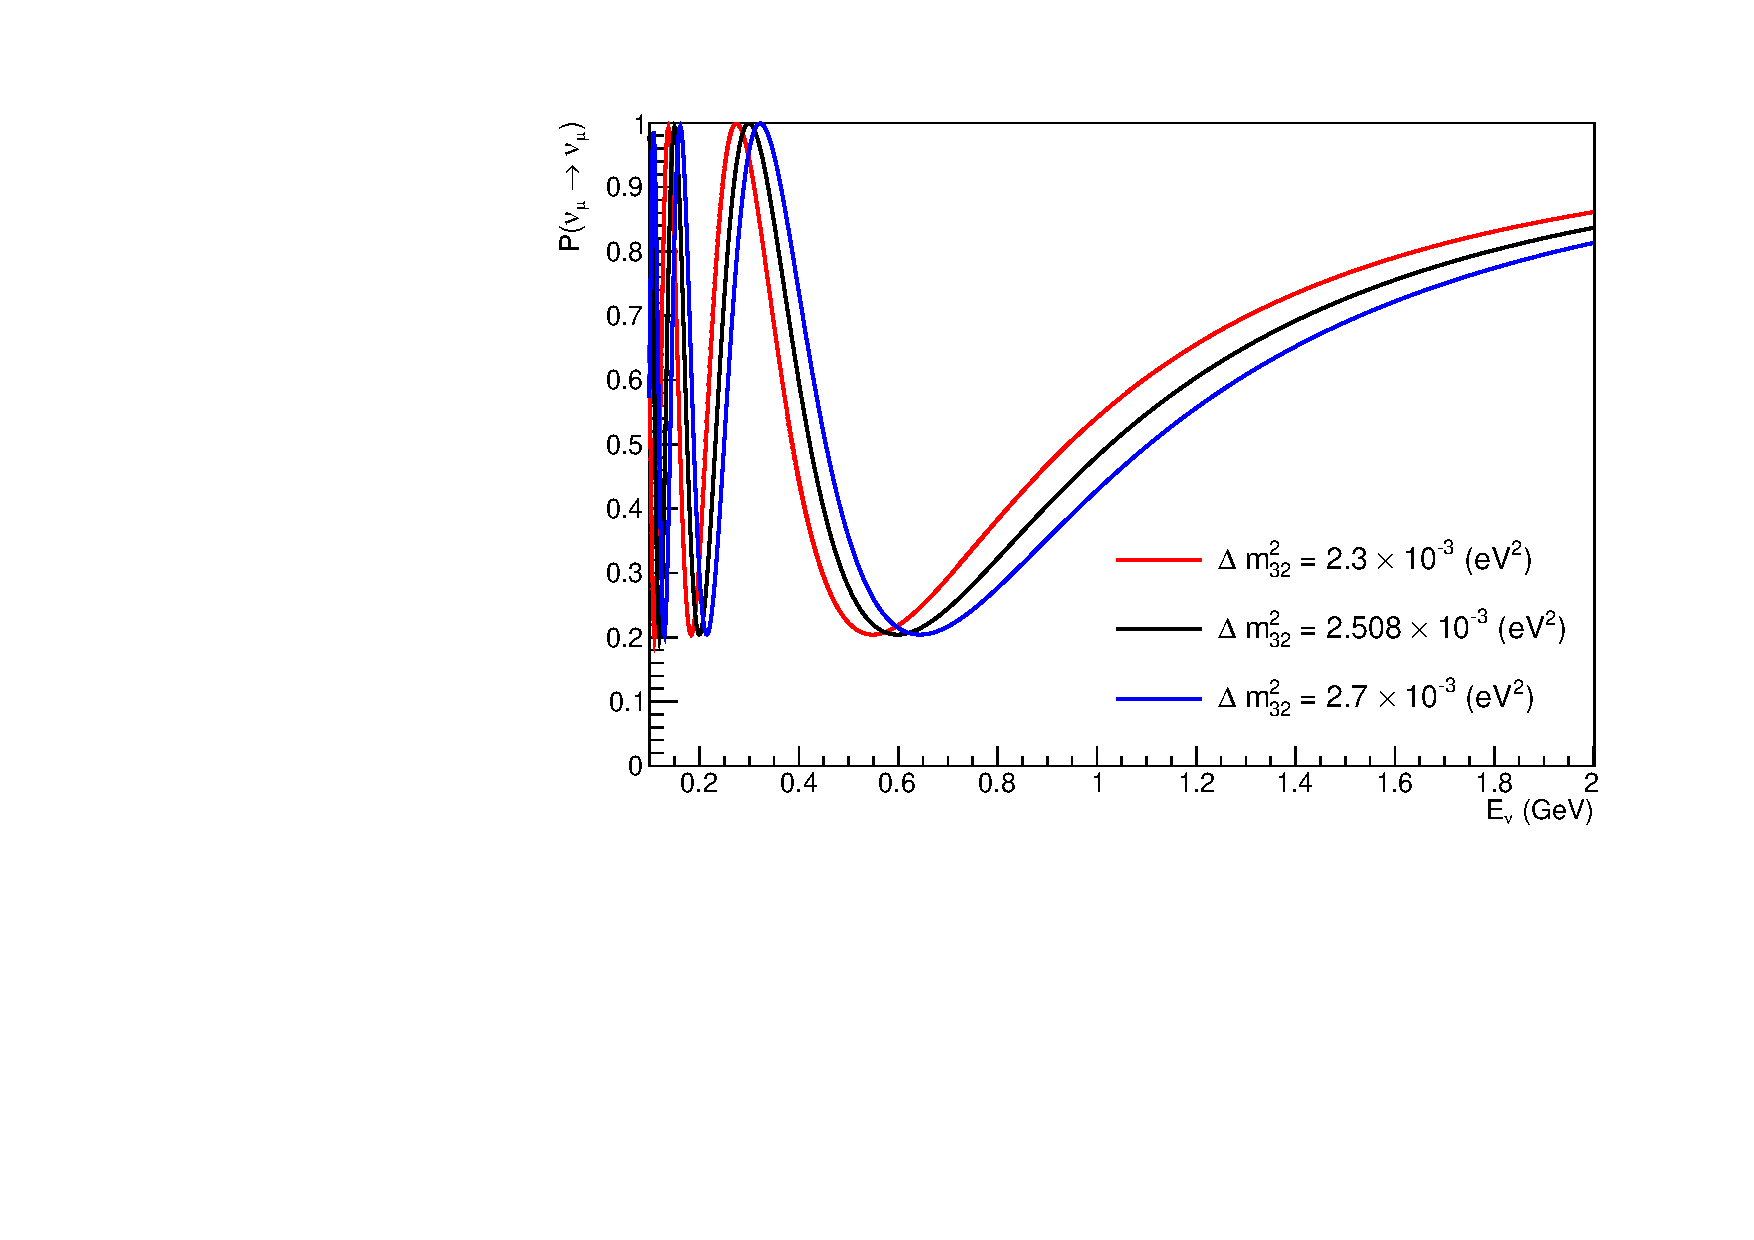
\includegraphics[width=\textwidth, trim={0mm 0mm 0mm 0mm}, clip,page=1]{Figures/Oscillation/T2K_NuMu_x_NuMu_DelMsq32Sens.pdf}
    \subcaption{\delmsqatm}
  \end{subfigure}%
  \begin{subfigure}[t]{0.5\textwidth}
    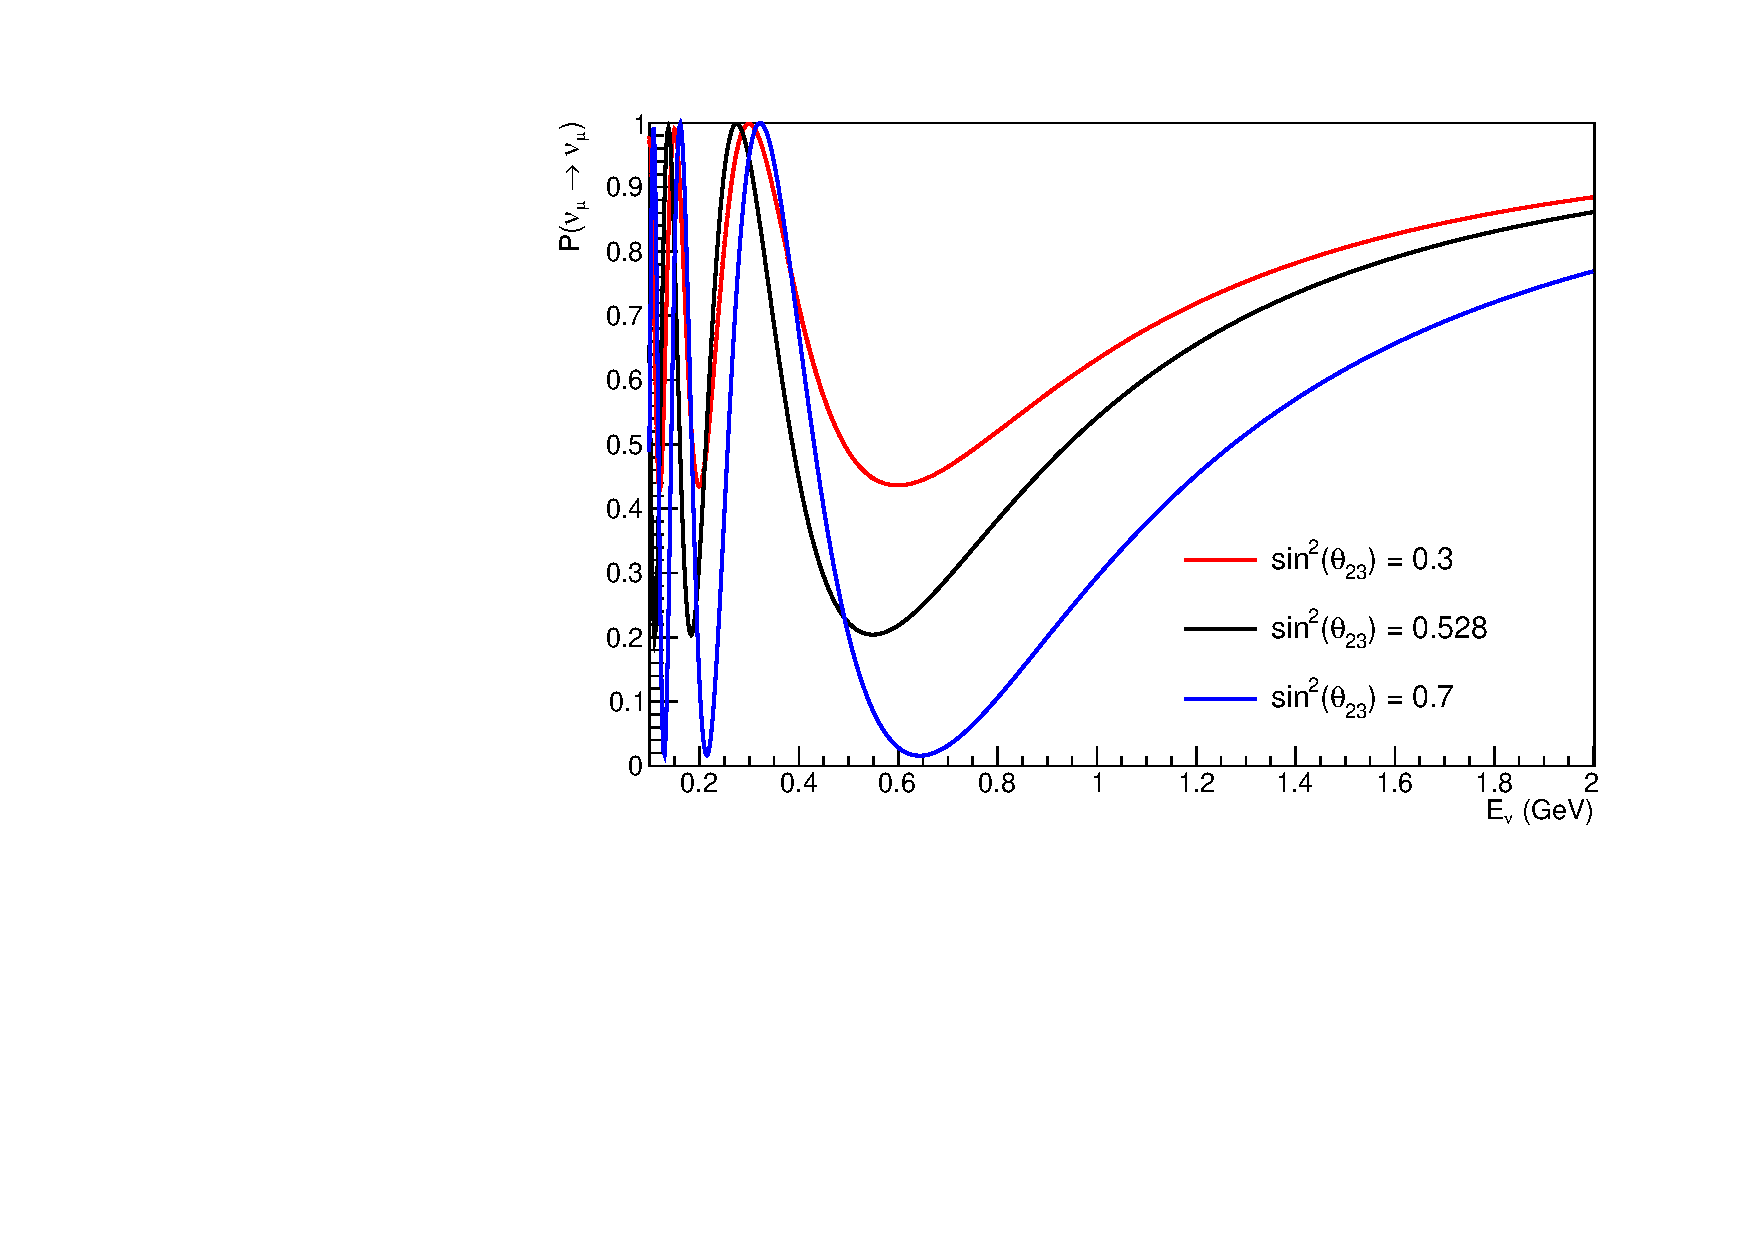
\includegraphics[width=\textwidth, trim={0mm 0mm 0mm 0mm}, clip,page=1]{Figures/Oscillation/T2K_NuMu_x_NuMu_Sinsqth23Sens.pdf}
    \subcaption{\sinsqatm}
  \end{subfigure}
  \begin{subfigure}[t]{0.5\textwidth}
    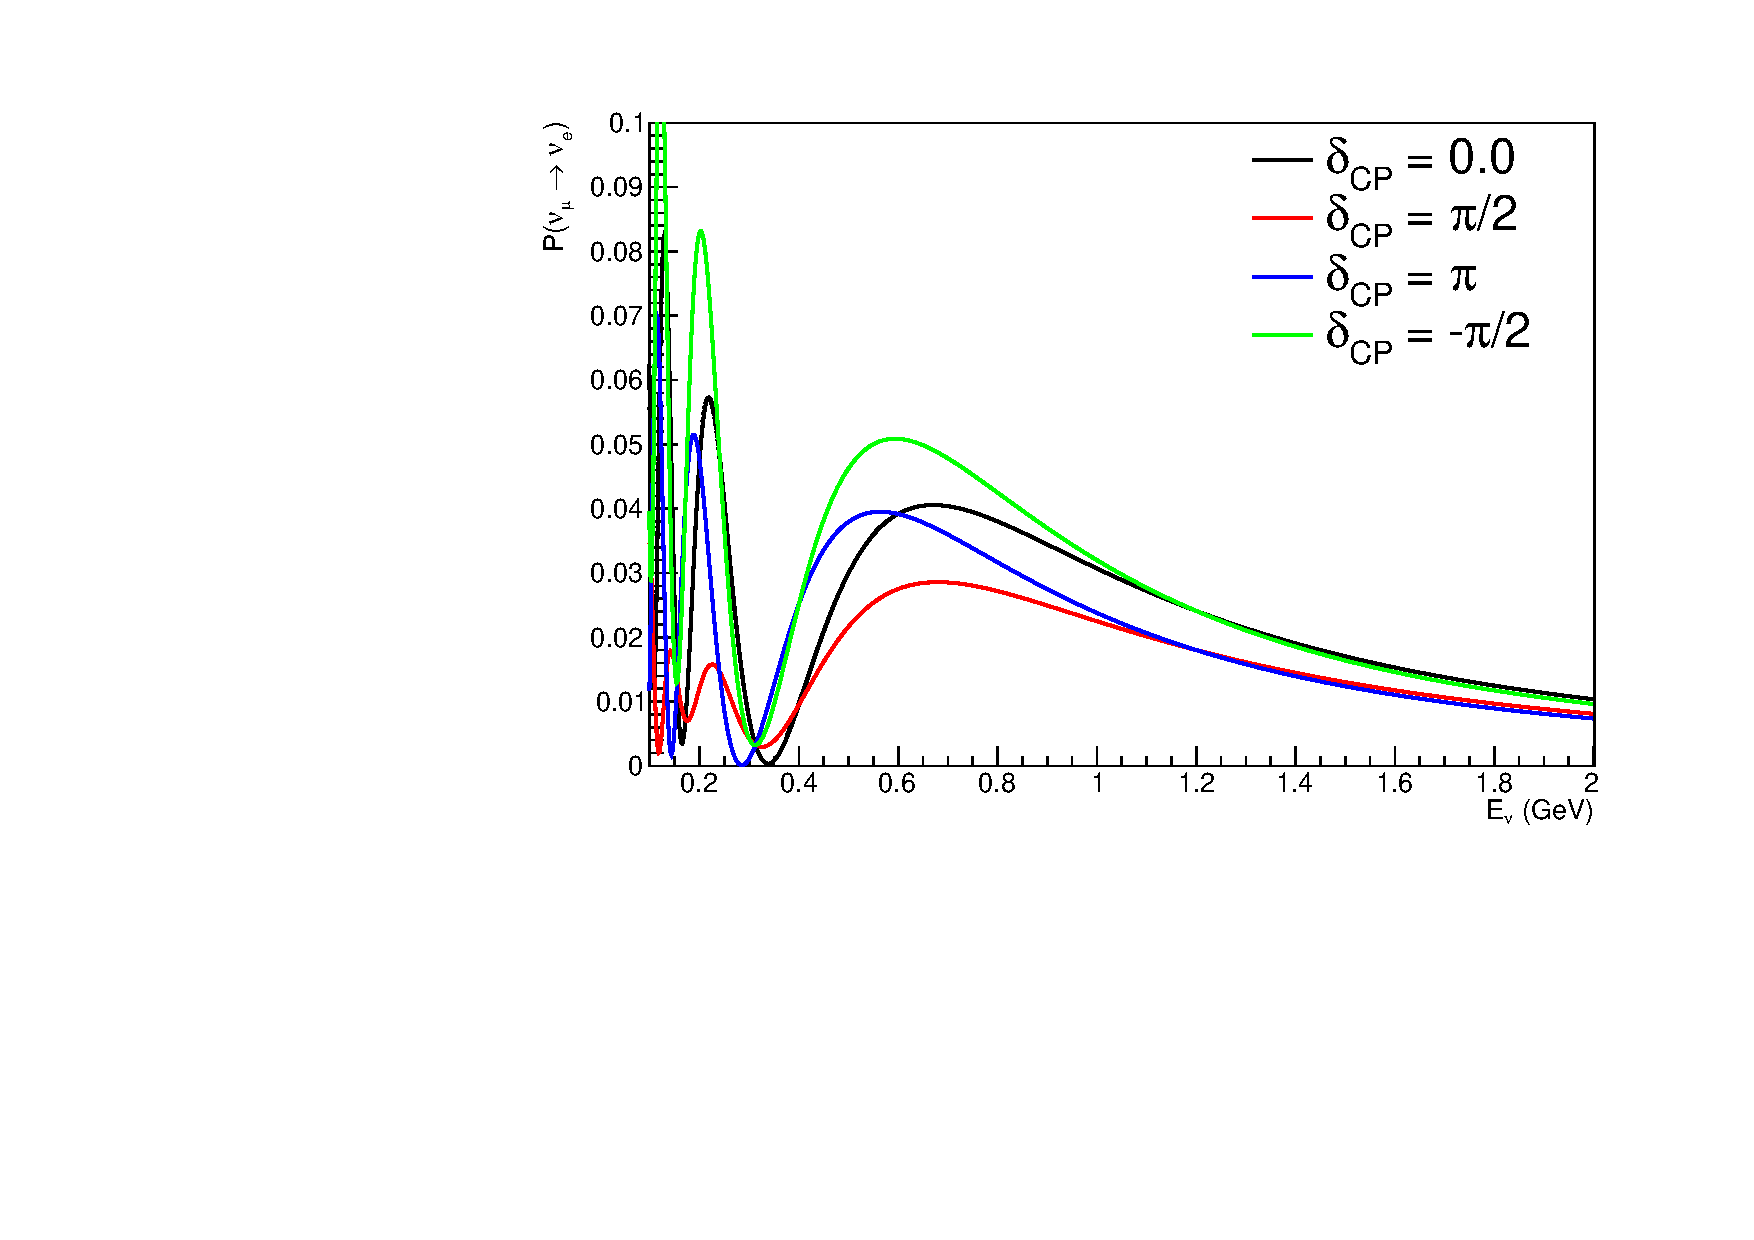
\includegraphics[width=\textwidth, trim={0mm 0mm 0mm 0mm}, clip,page=1]{Figures/Oscillation/T2K_NuMu_x_NuE_DCPSens.pdf}
    \subcaption{\dcp}
  \end{subfigure}
  \caption{}
  \label{fig:Oscillation_T2K_OscillationProbSensitivity}
\end{figure}
